%
% fig/dreieck-konstruktion.tex -- Konstruktion eines gleichseitigen
% Dreiecks aus zwei gegebenen Punkten durch Drehung um 60 Grad.
% Beispielwerte gemaess Praesentation: A=1+i, B=3+i, C=2+(1+sqrt3)i
%
\begin{figure}
\centering
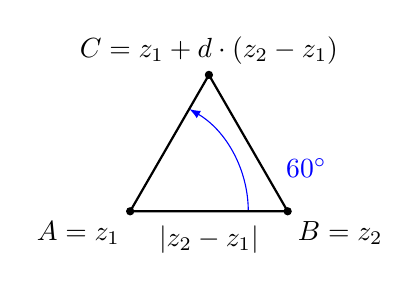
\begin{tikzpicture}[>=latex,thick,scale=1.0]
% Punkte (mit kleinem Offset, so dass A nicht im Ursprung liegt)
\coordinate (A) at (1.0, 1.0);
\coordinate (B) at (3.0, 1.0);
\coordinate (C) at (2.0, 2.732);
% Hilfslinien fuer den Drehwinkel
\draw[gray,thin,dashed] (A) -- (B);
\draw[gray,thin,dashed] (A) -- (C);
% Drehbogen von B um A nach C (Radius 2, Start 0 Grad, Ende 60 Grad)
\draw[->,blue,thin]
        (2.5,1.0) arc (0:60:1.5);
\node[blue] at (2.85,1.55) [right] {$60^\circ$};
% Dreieck
\draw[thick] (A) -- (B) -- (C) -- cycle;
% Eckpunkte
\fill (A) circle (1.5pt);
\fill (B) circle (1.5pt);
\fill (C) circle (1.5pt);
% Beschriftungen der Punkte
\node at (A) [below left]  {$A = z_1$};
\node at (B) [below right] {$B = z_2$};
\node at (C) [above]       {$C = z_1 + d \cdot (z_2 - z_1)$};
% Seitenlaengen
\node at (2.0,0.95) [below] {$|z_2 - z_1|$};
\end{tikzpicture}
\caption{Konstruktion des dritten Eckpunkts $C$ eines gleichseitigen
Dreiecks aus zwei gegebenen Punkten $A$ und $B$:
Drehung von $B$ um $A$ um den Winkel $60^\circ$ mit dem Drehfaktor
$d = \cos(60^\circ) + i \sin(60^\circ)$ ergibt $C$.
\label{komplex:figure:dreieck-konstruktion}}
\end{figure}
